\section{Discussion}
\label{sec:discuss}

In this section we perform further analysis on the clustering output
of our best model and indicate the possible reasons of comparably low
\vm\ scores.  To illustrate how words are distributed in the induced
clusters, we compare the output of our model with gold-tags of the
PTB.  We also discuss the effect of coarse gold-tag sets on our model
performance.
\begin{figure*}[ht] \centering
%\vspace*{-10mm}
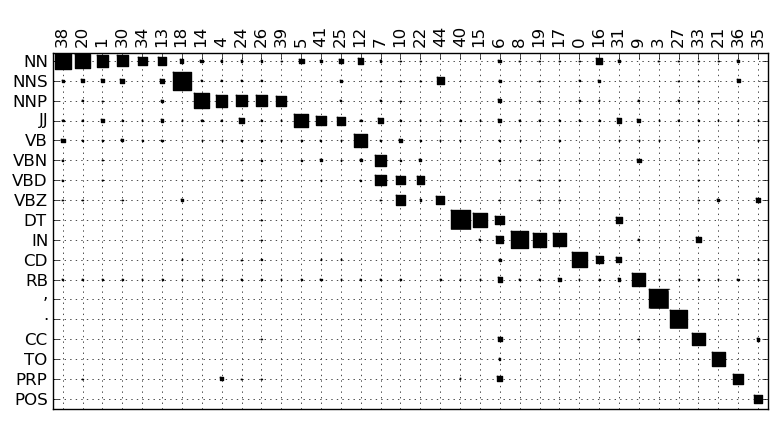
\includegraphics[width=\textwidth]{hinton.png}
%\vspace*{-30mm}
\caption{Hinton diagram comparing most frequent tags and clusters.
  Area of each square is proportional to the joint probability of the
  given tag and cluster.}
\label{plot-hinton}
\end{figure*}

Figure~\ref{plot-hinton} is the Hinton diagram of the PTB showing the
relationship between the most frequent tags and clusters from the
experiment in Section~\ref{sec:feat}.  In general the errors seem to
be the lack of completeness (multiple large entries in a row), rather
than lack of homogeneity (multiple large entries in a column).  The
algorithm tends to split large word classes into several clusters.
Some examples are:
\begin{itemize}
\item Titles like Mr., Mrs., and Dr. are split from the rest of the
  proper nouns in cluster (39).
\item Auxiliary verbs (10) and the verb ``say'' (22) have been split
  from the general verb clusters (12) and (7).
\item Determiners ``the'' (40), ``a'' (15), and capitalized
  ``The'', ``A'' (6) have been split into their own clusters.
\item Prepositions ``of'' (19), and ``by'', ``at'' (17) have been
  split from the general preposition cluster (8).
\end{itemize}
Nevertheless there are some homogeneity errors as well:
\begin{itemize} 
\item The adjective cluster (5) also has some noun members probably
  due to the difficulty of separating noun-noun compounds from
  adjective modification.
\item Cluster (6) contains capitalized words that span a number of
  categories.
\end{itemize}
%% A comparison of morphological structures might be helpful.
%% 
Most closed-class items are cleanly separated into their own clusters
as seen in the lower right hand corner of the diagram. 

The completeness errors become more noticeable on languages with
coarse tag-sets thus our models perform worse than the best published
models on 6 of MULTEXT-East languages in terms of \vm\ scores while
achieving the state-of-the-art \mto\ scores on same languages as shown
on Table~\ref{tab:multiresults}.  On CONLL-X languages the effect of
completeness errors is less noticeable since all languages except
Czech and Dutch have fine grained tag-sets.

The completeness errors are not surprising given that the words that
have been split are not generally substitutable with the other members
of their gold-tag set category.  Thus it can be argued that metrics
that emphasize homogeneity such as \mto\ are more appropriate in this
context than metrics that average homogeneity and completeness such as
\vm\ as long as the number of clusters is controlled.

